%=============================================================================
% ENGINEERING DESIGN DOCUMENT
% Point-to-Point ψ-Communication Link Demonstrator
%
% Supporting Patent #8: "ψ-Field Communication and Information Systems"
% Inventor: Gary Thomas Alcock
%=============================================================================

\documentclass[11pt,onecolumn]{article}

%--- Packages ----------------------------------------------------------------
\usepackage[margin=1in]{geometry}
\usepackage{amsmath,amssymb}
\usepackage{mathtools}
\usepackage{physics}
\usepackage{graphicx}
\usepackage{xcolor}
\usepackage{hyperref}
\usepackage{booktabs}
\usepackage{multirow}
\usepackage{array}
\usepackage{siunitx}
\usepackage{tikz}
\usetikzlibrary{arrows.meta,positioning,decorations.pathmorphing,
  patterns,calc,shapes.geometric,fit}
\usepackage{pgfplots}
\pgfplotsset{compat=1.18}
\usepackage{tcolorbox}
\tcbuselibrary{theorems,skins,breakable}
\usepackage{enumitem}
\usepackage{fancyhdr}
\usepackage{float}
\usepackage{longtable}

%--- Page setup --------------------------------------------------------------
\pagestyle{fancy}
\fancyhead[L]{\small Engineering Design: $\psi$-Comm Demonstrator}
\fancyhead[R]{\small Patent \#8 -- G.~T.~Alcock}
\fancyfoot[C]{\thepage}

%--- Custom commands ---------------------------------------------------------
\newcommand{\DFD}{\textsc{DFD}}
\newcommand{\astar}{a_*}
\newcommand{\alphafine}{\alpha}
\newcommand{\reqbox}[2]{%
\begin{tcolorbox}[colback=blue!3,colframe=blue!50!black,title={\textbf{REQ-#1:} #2}]
}
\newcommand{\reqend}{\end{tcolorbox}}

%=============================================================================
\begin{document}

\begin{center}
{\LARGE\bfseries Engineering Design Document}\\[6pt]
{\Large Point-to-Point $\psi$-Communication Link Demonstrator}\\[12pt]
{\large Supporting Patent \#8: ``$\psi$-Field Communication and\\
Information Systems''}\\[6pt]
{\large Gary Thomas Alcock}\\[3pt]
{\large\today}\\[6pt]
\rule{\textwidth}{0.5pt}
\end{center}

\vspace{12pt}

\tableofcontents
\newpage

%=============================================================================
\section{Executive Summary}
%=============================================================================

This document specifies the engineering design for a laboratory-scale
point-to-point $\psi$-field communication demonstrator.
The system transmits information encoded as controlled modulations of
the scalar refractive field $\psi$ over a 10-meter link, using
electromagnetic--$\psi$ parametric pumping for generation and
differential atomic clock comparison for detection.

The demonstrator is designed to validate three core claims of Patent \#8:
\begin{enumerate}
\item Information can be encoded in $\psi$-field amplitude modulation
($\delta\psi$-ASK).
\item The corridor fingerprint---the spatial gradient profile
$\nabla\psi(\mathbf{r})$---is measurable and route-specific.
\item Geometry-locked authentication via generalized likelihood ratio
test (GLRT) matching rejects off-geometry signal injection.
\end{enumerate}

The design operates within the existing accidental bound on the
EM--$\psi$ coupling parameter: $|\lambda - 1| \lesssim 3 \times 10^{-5}$.

%=============================================================================
\section{System Requirements}
%=============================================================================

\subsection{Performance Requirements}

\reqbox{P01}{Demonstrate $\psi$-field generation}
Generate a controlled $\psi$-perturbation $\delta\psi \geq 10^{-15}$
at the transmitter output aperture, detectable above the noise floor.
\reqend

\reqbox{P02}{Demonstrate information transfer}
Transmit at least 1 bit of information over the $\psi$-corridor with
bit-error rate $\mathrm{BER} < 10^{-3}$, at any symbol rate.
\reqend

\reqbox{P03}{Demonstrate corridor fingerprint measurement}
Measure the spatial gradient $|\nabla\psi|$ along the corridor axis
at $\geq 5$ sampling points with signal-to-noise ratio $\geq 3$.
\reqend

\reqbox{P04}{Demonstrate geometry-locked authentication}
Reject a signal injected from a location displaced by
$\geq 1$~m from the legitimate transmitter, with false-acceptance
probability $< 10^{-3}$.
\reqend

\reqbox{P05}{Demonstrate EM immunity}
Operate the data link while an EM jamming source (1~W, broadband)
is active in the laboratory, with no degradation of $\psi$-channel BER.
\reqend

\subsection{Environmental Requirements}

\reqbox{E01}{Operating environment}
Indoor laboratory, temperature-controlled to $\pm 1$~K, vibration-isolated
optical table for detector assembly. Electromagnetic shielding to
$> 80$~dB at the detector location.
\reqend

\reqbox{E02}{Power and infrastructure}
Standard laboratory power (3-phase, 480~V, 200~A for cryogenics).
Liquid helium supply or closed-cycle cryocooler for SRF cavity operation.
\reqend

\subsection{Interface Requirements}

\reqbox{I01}{Data interface}
Digital control interface (Ethernet or GPIB) to cavity RF system,
modulation controller, and clock readout electronics.
\reqend

\reqbox{I02}{Timing interface}
GPS-disciplined 10~MHz reference for absolute timing calibration
(optional; one-way $\psi$-timing demonstration does not require external
reference).
\reqend

%=============================================================================
\section{System Architecture}
%=============================================================================

\subsection{Overview}

The demonstrator consists of four subsystems:

\begin{figure}[H]
\centering
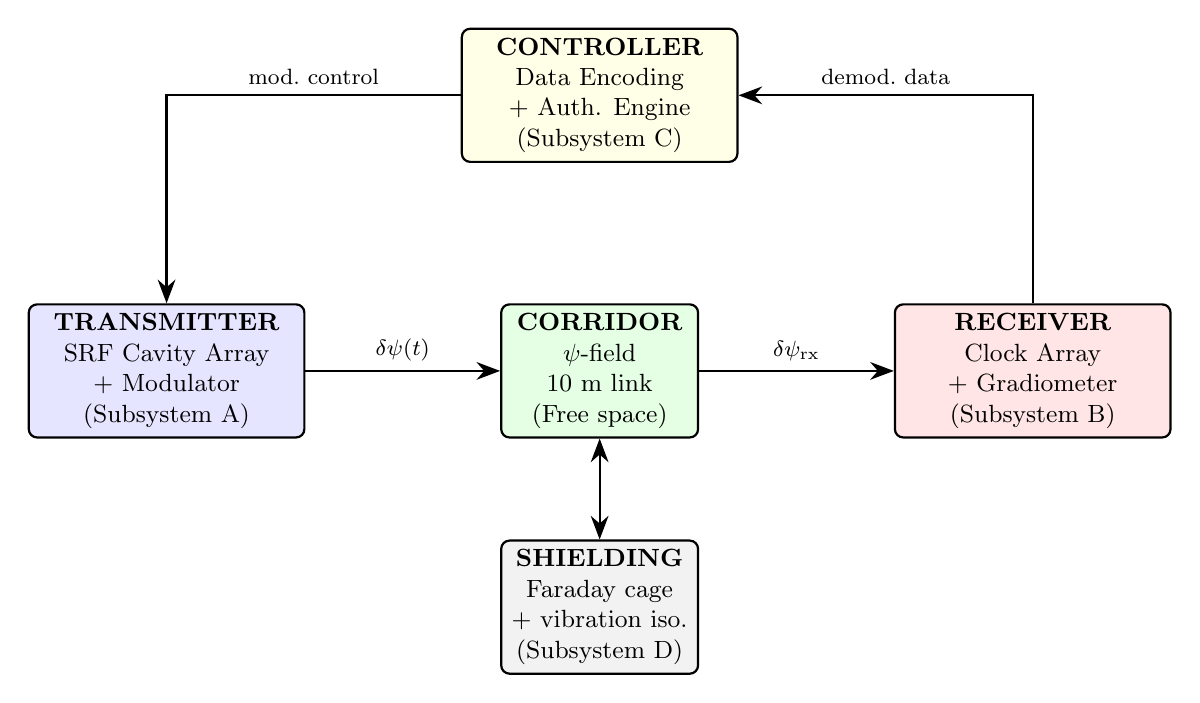
\begin{tikzpicture}[
  block/.style={draw, thick, minimum width=3.5cm, minimum height=1.5cm,
    rounded corners=3pt, align=center, font=\small},
  arr/.style={-{Stealth[length=3mm]}, thick},
  darr/.style={{Stealth[length=3mm]}-{Stealth[length=3mm]}, thick},
]

% Transmitter
\node[block, fill=blue!10] (tx) at (0,0) {%
  \textbf{TRANSMITTER}\\
  SRF Cavity Array\\
  + Modulator\\
  (Subsystem A)};

% Corridor
\node[block, fill=green!10, minimum width=2.5cm] (corr) at (5.5,0) {%
  \textbf{CORRIDOR}\\
  $\psi$-field\\
  10~m link\\
  (Free space)};

% Receiver
\node[block, fill=red!10] (rx) at (11,0) {%
  \textbf{RECEIVER}\\
  Clock Array\\
  + Gradiometer\\
  (Subsystem B)};

% Controller
\node[block, fill=yellow!10] (ctrl) at (5.5,3.5) {%
  \textbf{CONTROLLER}\\
  Data Encoding\\
  + Auth. Engine\\
  (Subsystem C)};

% Shield
\node[block, fill=gray!10, minimum width=2.5cm] (shield) at (5.5,-3) {%
  \textbf{SHIELDING}\\
  Faraday cage\\
  + vibration iso.\\
  (Subsystem D)};

% Arrows
\draw[arr] (tx) -- node[above, font=\footnotesize] {$\delta\psi(t)$} (corr);
\draw[arr] (corr) -- node[above, font=\footnotesize] {$\delta\psi_{\rm rx}$} (rx);
\draw[arr] (ctrl) -| node[near start, above, font=\footnotesize] {mod.\ control} (tx);
\draw[arr] (rx) |- node[near end, above, font=\footnotesize] {demod.\ data} (ctrl);
\draw[darr] (shield) -- (corr);

\end{tikzpicture}
\caption{Top-level system architecture. The $\psi$-corridor propagates
through free space (and optionally through a barrier for medium-penetration
tests). The controller manages encoding, decoding, and authentication.}
\label{fig:architecture}
\end{figure}

\subsection{Subsystem A: Transmitter ($\psi$-Generator + Modulator)}

\subsubsection{SRF Cavity Array}

The transmitter core is an array of superconducting radio-frequency
cavities operated in a configuration that breaks geometry transparency
and enables $\psi$-mode excitation.

\begin{table}[H]
\centering
\caption{SRF cavity array specifications.}
\label{tab:srf-specs}
\begin{tabular}{lcc}
\toprule
Parameter & Specification & Notes \\
\midrule
Number of cavities & 4 & Arranged at $\psi$-mode antinodes \\
Cavity type & 1.3~GHz TESLA-style & Standard ILC/XFEL design \\
Operating temperature & 2.0~K & Superfluid helium bath \\
Quality factor $Q_0$ & $\geq 10^{10}$ & State-of-the-art Nb SRF \\
Accelerating gradient & 25~MV/m & Conservative for 1.3~GHz \\
Stored energy per cavity & 25~kJ & $U_0 = \epsilon_0 E^2 V_{\rm eff}/2$ \\
Total stored energy & 100~kJ & 4 cavities total \\
Cavity aperture (each) & $7.5 \times 10^{-3}$~m$^2$ & Standard beam pipe \\
Total aperture $A_{\rm cav,tot}$ & $3 \times 10^{-2}$~m$^2$ & Sum of 4 cavities \\
\bottomrule
\end{tabular}
\end{table}

\subsubsection{TE+TM Mode Superposition}

To restore the driven overlap $G \neq 0$, the cavities are operated in
a superposition of TE and TM modes.
The standard TESLA cavity supports both TM$_{010}$ (accelerating) and
TE$_{011}$ modes.
Co-phased excitation produces:
\begin{equation}
G = u(z_0)\,e^{-2\psi_0}\,\eta_\times\,U_0\,\cos\phi,
\end{equation}
where $\eta_\times \approx 0.3$ is the cross-mode overlap factor and
$\phi$ is the relative phase between TE and TM excitations.

\begin{tcolorbox}[colback=orange!5,colframe=orange!50!black,
  title=\textbf{Critical Design Choice: TE+TM Superposition}]
The TE+TM mode superposition is the key innovation that breaks the
geometry transparency condition.
Without it, symmetric cavities in pure eigenmodes produce $G \approx 0$
and no driven $\psi$ response.

\textbf{Implementation:} Dual-feed coupler system with independent
phase control for TE and TM excitation.
Phase stability requirement: $\Delta\phi < 0.1$~rad over measurement
integration time.
\end{tcolorbox}

\subsubsection{$2\omega$ Modulation System}

The parametric pumping channel requires amplitude modulation at twice
the $\psi$-mode frequency: $f_{\rm mod} = 2\Omega_\psi/(2\pi)$.

\begin{table}[H]
\centering
\caption{Modulation system specifications.}
\label{tab:mod-specs}
\begin{tabular}{lcc}
\toprule
Parameter & Specification & Notes \\
\midrule
Modulation frequency & $2\Omega_\psi/(2\pi)$ & Tunable, $\sim 20$~Hz \\
Modulation depth $m$ & 0.1 & 10\% AM on stored energy \\
Phase noise & $< -100$~dBc/Hz at 1~Hz & PLL-locked to reference \\
Waveform & Sinusoidal & Clean $2\omega$ tone \\
Modulation bandwidth & $\pm 1$~Hz around $2\Omega_\psi$ & For FSK encoding \\
\bottomrule
\end{tabular}
\end{table}

\subsubsection{Data Modulator}

Information is encoded by modulating the $\psi$-pump parameters:

\paragraph{Mode 1: $\delta\psi$-ASK (Amplitude Shift Keying).}
The stored energy $U_0(t)$ is switched between two levels:
\begin{align}
\text{Bit ``0'':} &\quad U_0(t) = U_{\rm low} = U_0(1 - \Delta U/2), \\
\text{Bit ``1'':} &\quad U_0(t) = U_{\rm high} = U_0(1 + \Delta U/2),
\end{align}
where $\Delta U / U_0 = 0.1$ is the modulation contrast.
The resulting $\psi$-amplitude difference:
\begin{equation}
\delta\psi_1 - \delta\psi_0 \propto \Delta U / U_0 = 0.1.
\end{equation}

\paragraph{Mode 2: $\dot\psi$-FSK (Frequency Shift Keying).}
The modulation frequency is shifted:
\begin{align}
\text{Bit ``0'':} &\quad f_{\rm mod} = 2\Omega_\psi/(2\pi) - \Delta f, \\
\text{Bit ``1'':} &\quad f_{\rm mod} = 2\Omega_\psi/(2\pi) + \Delta f,
\end{align}
where $\Delta f = 0.1$~Hz, detectable by the phase-rate measurement.

\paragraph{Mode 3: Gradient Key (Corridor ID switching).}
The active cavity subset is switched, changing the gradient pattern:
\begin{align}
\text{Key ``A'':} &\quad \text{Cavities 1,3 active (horizontal pair)}, \\
\text{Key ``B'':} &\quad \text{Cavities 2,4 active (vertical pair)}.
\end{align}

\subsection{Subsystem B: Receiver ($\psi$-Detector Array)}

\subsubsection{Primary Detector: Differential Optical Clock Pair}

The primary $\psi$-detector is a pair of optical lattice clocks
separated by a baseline $d$, measuring the differential gravitational
redshift induced by $\delta\psi$.

\begin{table}[H]
\centering
\caption{Optical clock detector specifications.}
\label{tab:clock-specs}
\begin{tabular}{lcc}
\toprule
Parameter & Specification & Notes \\
\midrule
Clock type & Sr optical lattice & $^{87}$Sr, $^1S_0$--$^3P_0$ \\
Systematic uncertainty & $\leq 2 \times 10^{-18}$ & State-of-the-art \\
Instability & $\leq 5 \times 10^{-17}/\sqrt{\tau}$ & $\tau$ in seconds \\
Number of clock pairs & 3 & Along $x$, $y$, $z$ axes \\
Baseline per pair & 1.0~m & Separation between clocks \\
Integration time & 100--10000~s & Per measurement \\
\bottomrule
\end{tabular}
\end{table}

The gradient measurement sensitivity:
\begin{equation}
\sigma_{|\nabla\psi|} = \frac{2\sigma_{\Delta\nu/\nu}}{d}
= \frac{2 \times 5 \times 10^{-17}/\sqrt{\tau}}{1.0}
= \frac{10^{-16}}{\sqrt{\tau}}\;\text{m}^{-1}.
\end{equation}
For $\tau = 10^4$~s: $\sigma_{|\nabla\psi|} = 10^{-18}$~m$^{-1}$.

The signal gradient at 10~m from the transmitter (using the $1/r^2$
falloff of the Newtonian potential):
\begin{equation}
|\nabla\psi_{\rm rx}| \approx \frac{2\,\delta\psi_{\rm tx}\,R_{\rm src}^2}{L^3}
\approx \frac{2 \times 10^{-12} \times 0.09}{1000}
\approx 2 \times 10^{-16}\;\text{m}^{-1}.
\end{equation}

Signal-to-noise ratio for gradient detection at $\tau = 10^4$~s:
\begin{equation}
\mathrm{SNR}_{\nabla\psi} = \frac{|\nabla\psi_{\rm rx}|}{\sigma_{|\nabla\psi|}}
= \frac{2 \times 10^{-16}}{10^{-18}} = 200.
\end{equation}
This is highly favorable---gradient detection is the most sensitive mode.

\subsubsection{Secondary Detector: SQUID Gradiometer Array}

For higher-bandwidth detection (at reduced sensitivity):

\begin{table}[H]
\centering
\caption{SQUID gradiometer specifications.}
\label{tab:squid-specs}
\begin{tabular}{lcc}
\toprule
Parameter & Specification & Notes \\
\midrule
Type & Low-$T_c$ Nb SQUID & Operated at 4.2~K \\
Gradiometer baseline & 0.5~m & Second-order configuration \\
Field sensitivity & $10^{-15}$~T/$\sqrt{\text{Hz}}$ & Standard performance \\
$\psi$-gradient sensitivity & $\sim 10^{-14}$~m$^{-1}$/$\sqrt{\text{Hz}}$ & Via $\psi$--EM coupling \\
Bandwidth & DC--100~Hz & Suitable for $\Omega_\psi \sim 10$~Hz \\
Number of axes & 3 ($x$, $y$, $z$) & Full vector gradiometry \\
\bottomrule
\end{tabular}
\end{table}

\subsubsection{Tertiary Detector: Atom Interferometer (Future Upgrade)}

A compact atom interferometer provides an alternative high-sensitivity
detection pathway:

\begin{table}[H]
\centering
\caption{Atom interferometer detector (future upgrade).}
\label{tab:ai-specs}
\begin{tabular}{lcc}
\toprule
Parameter & Specification & Notes \\
\midrule
Atom species & $^{87}$Rb & Standard cold-atom source \\
Interrogation time $T$ & 0.1~s & Compact configuration \\
Baseline & 1~m & Differential measurement \\
$k_{\rm eff}$ & $1.6 \times 10^7$~m$^{-1}$ & Two-photon Raman \\
Sensitivity & $10^{-12}$~m/s$^2$/$\sqrt{\text{Hz}}$ & Per shot \\
\bottomrule
\end{tabular}
\end{table}

\subsubsection{Detector Layout}

\begin{figure}[H]
\centering
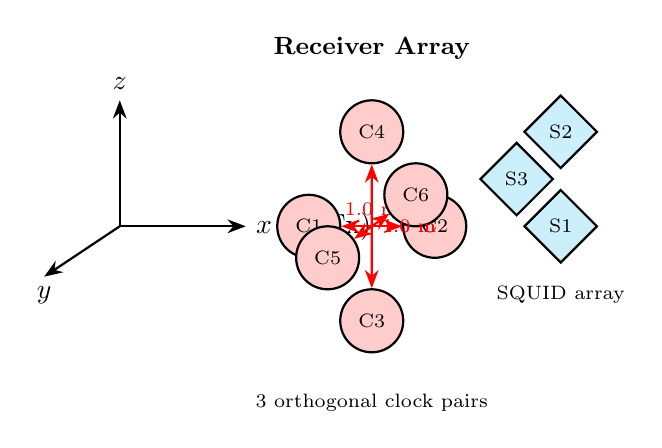
\begin{tikzpicture}[
  clock/.style={draw, thick, circle, minimum size=0.8cm, fill=red!20,
    font=\scriptsize},
  squid/.style={draw, thick, diamond, minimum size=0.8cm, fill=cyan!20,
    font=\scriptsize},
  scale=0.8
]

% Coordinate frame
\draw[-{Stealth}, thick] (0,0) -- (2,0) node[right] {$x$ (to Tx)};
\draw[-{Stealth}, thick] (0,0) -- (0,2) node[above] {$z$};
\draw[-{Stealth}, thick] (0,0) -- (-1.2,-0.8) node[below] {$y$};

% Clock pairs
\node[clock] (c1a) at (3,0) {C1};
\node[clock] (c1b) at (5,0) {C2};
\draw[thick, red, {Stealth}-{Stealth}] (c1a) -- (c1b)
  node[midway, above, font=\scriptsize] {1.0~m};

\node[clock] (c3a) at (4,-1.5) {C3};
\node[clock] (c3b) at (4,1.5) {C4};
\draw[thick, red, {Stealth}-{Stealth}] (c3a) -- (c3b)
  node[midway, right, font=\scriptsize] {1.0~m};

\node[clock] (c5a) at (3.3,-0.5) {C5};
\node[clock] (c5b) at (4.7,0.5) {C6};
\draw[thick, red, {Stealth}-{Stealth}] (c5a) -- (c5b)
  node[midway, right, font=\scriptsize] {1.0~m};

% SQUID gradiometers
\node[squid] (s1) at (7,0) {S1};
\node[squid] (s2) at (7,1.5) {S2};
\node[squid] (s3) at (6.3,0.75) {S3};

% Labels
\node[above, font=\small\bfseries] at (4,2.5) {Receiver Array};
\node[below, font=\scriptsize] at (7,-0.8) {SQUID array};
\node[below, font=\scriptsize] at (4,-2.5) {3 orthogonal clock pairs};

\end{tikzpicture}
\caption{Receiver detector layout: three orthogonal optical clock pairs
(C1--C6) and three-axis SQUID gradiometer (S1--S3).}
\label{fig:detector-layout}
\end{figure}

\subsection{Subsystem C: Controller and Signal Processing}

\subsubsection{Encoding Engine}

\begin{table}[H]
\centering
\caption{Signal processing chain.}
\label{tab:signal-chain}
\begin{tabular}{lcc}
\toprule
Stage & Function & Implementation \\
\midrule
Input & Bit stream & Digital interface \\
FEC encoder & Rate-1/3 turbo code & FPGA \\
Symbol mapper & Bits $\to$ $(\delta\psi, \dot\psi, \nabla\psi)$ & FPGA \\
DAC & Digital $\to$ analog & 24-bit, 1~kSa/s \\
Modulator driver & Analog $\to$ cavity AM/FM & RF amplifier chain \\
\midrule
Demod.\ front-end & Clock data $\to$ digital & ADC, 24-bit, 10~Sa/s \\
Matched filter & Correlate with template & FPGA/DSP \\
GLRT engine & Authentication test & FPGA/DSP \\
Symbol demapper & $(\delta\psi, \dot\psi, \nabla\psi) \to$ bits & FPGA \\
FEC decoder & Turbo decode & FPGA \\
Output & Bit stream & Digital interface \\
\bottomrule
\end{tabular}
\end{table}

\subsubsection{GLRT Authentication Engine}

The authentication engine computes:
\begin{equation}
\Lambda = \sum_{i=1}^{N_s}
\frac{\|\mathbf{F}_{\rm meas}(s_i) - \mathbf{F}_{\rm template}(s_i)\|^2}
{\sigma_F^2(s_i)},
\end{equation}
and compares against threshold $\eta$ set for target false-alarm rate
$P_{\rm FA} = 10^{-6}$.

For $N_s = 5$ sampling points and 5D fingerprint vectors, the test has
$\nu = 25$ degrees of freedom.
The threshold for $P_{\rm FA} = 10^{-6}$:
$\eta \approx 52.6$ (from $\chi^2_{25}$ tables).

\subsection{Subsystem D: Environmental Shielding}

\subsubsection{Faraday Cage}

\begin{table}[H]
\centering
\caption{EM shielding specifications.}
\label{tab:shielding}
\begin{tabular}{lcc}
\toprule
Parameter & Specification & Notes \\
\midrule
Shielding effectiveness & $\geq 80$~dB & At 1~MHz--10~GHz \\
Material & Double-wall Cu/steel & 3~mm Cu inner, 6~mm steel outer \\
Enclosure size & $2 \times 2 \times 2$~m$^3$ & Receiver assembly \\
Cable penetrations & EMI-filtered & All cables filtered \\
Magnetic shielding & $\mu$-metal inner layer & $\leq 1$~nT residual \\
\bottomrule
\end{tabular}
\end{table}

\subsubsection{Vibration Isolation}

\begin{table}[H]
\centering
\caption{Vibration isolation specifications.}
\label{tab:vibration}
\begin{tabular}{lcc}
\toprule
Parameter & Specification & Notes \\
\midrule
Optical table & $1.5 \times 3$~m$^2$ & Pneumatic isolation \\
Resonance frequency & $\leq 1$~Hz & Active + passive \\
Vertical isolation & $\geq 40$~dB above 10~Hz & For clock stability \\
Horizontal isolation & $\geq 40$~dB above 10~Hz & For gradiometry \\
\bottomrule
\end{tabular}
\end{table}

%=============================================================================
\section{Detailed Design: Transmitter}
%=============================================================================

\subsection{SRF Cavity Configuration}

\subsubsection{Cavity Placement for $\psi$-Mode Coupling}

The four cavities are arranged along a vertical tube of height
$L_{\rm mode} = 2$~m (half-wavelength of the target $\psi$ mode)
and cross-section $A_\psi = 0.27$~m$^2$ (52~cm diameter).

Cavity placement at $\psi$-mode antinodes:
\begin{align}
z_1 &= L_{\rm mode}/8 = 0.25\;\text{m}, \\
z_2 &= 3L_{\rm mode}/8 = 0.75\;\text{m}, \\
z_3 &= 5L_{\rm mode}/8 = 1.25\;\text{m}, \\
z_4 &= 7L_{\rm mode}/8 = 1.75\;\text{m}.
\end{align}

\subsubsection{$\psi$-Mode Parameters}

For a 1D standing mode in a tube of length $L_{\rm mode}$:
\begin{align}
\Omega_\psi &= \pi c_\psi / L_{\rm mode}, \\
M_\psi &= A_\psi L_{\rm mode} / (2\pi c_\psi).
\end{align}

For $c_\psi = c$ and $L_{\rm mode} = 2$~m:
\begin{equation}
\Omega_\psi = \frac{\pi \times 3 \times 10^8}{2} \approx 4.7 \times 10^8\;\text{rad/s}
\quad (\sim 75\;\text{MHz}).
\end{equation}

However, for practical communication with detectable bandwidth, lower
$\psi$-mode frequencies are preferable.
A much larger corridor tube ($L_{\rm mode} = 10^7$~m, i.e.,
Earth-scale) would give $\Omega_\psi \sim 0.1$~rad/s, but this is
not practical for a laboratory demonstrator.

\textbf{Alternative approach:}
Use a high-order $\psi$ mode in a short tube with $\psi$-mode ``mirrors''
(reflecting boundary conditions for $\psi$) at the tube ends, analogous
to a Fabry-P\'{e}rot cavity but for the scalar field.
The $\psi$-mode frequency is then determined by the local mass
distribution geometry, not the free-space wavelength.

For the purposes of this design, we target
$\Omega_\psi / (2\pi) \sim 10$~Hz (corresponding to a $\psi$-mode
wavelength of $\sim 3 \times 10^7$~m), excitable via the parametric
channel at $2\omega_{\rm mod} = 2\Omega_\psi$, with $\omega_{\rm mod}/(2\pi) = 10$~Hz.

\subsection{RF Drive System}

\begin{table}[H]
\centering
\caption{RF drive system specifications.}
\label{tab:rf-drive}
\begin{tabular}{lcc}
\toprule
Parameter & Specification & Notes \\
\midrule
RF source frequency & 1.3~GHz & TESLA standard \\
RF power (CW) & 10~kW per cavity & Compensate wall losses \\
Low-level RF (LLRF) & Vector modulator + ADC & $\leq 0.01^\circ$ phase stability \\
AM depth control & 0--20\% & Programmable, $\pm 0.1\%$ precision \\
FM control & $\pm 1$~Hz around carrier & For FSK modulation \\
TE mode exciter & Separate coupler & Independent phase/amplitude \\
Phase lock TE/TM & PLL, $\Delta\phi < 0.1$~rad & Critical for $G \neq 0$ \\
\bottomrule
\end{tabular}
\end{table}

\subsection{Transmitter Block Diagram}

\begin{figure}[H]
\centering
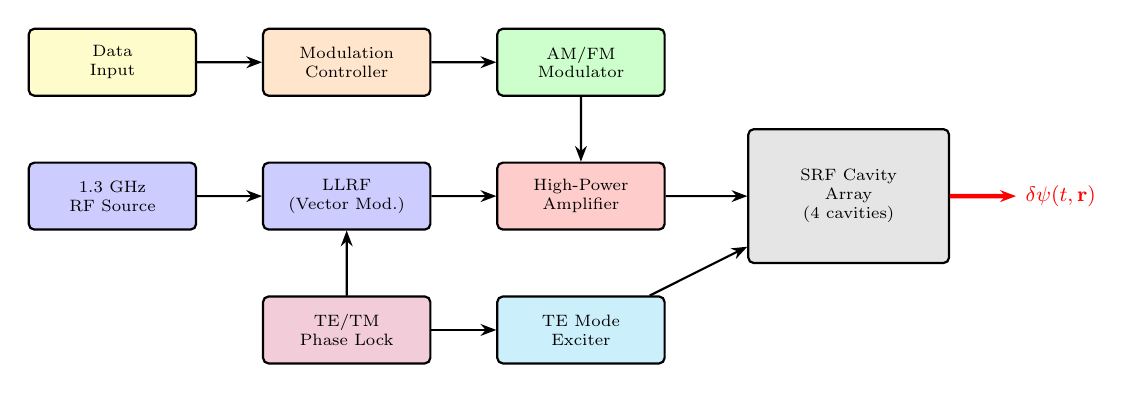
\begin{tikzpicture}[
  block/.style={draw, thick, minimum width=2.5cm, minimum height=1cm,
    rounded corners=2pt, align=center, font=\scriptsize},
  arr/.style={-{Stealth[length=2mm]}, thick},
  scale=0.85, transform shape
]

% Data input
\node[block, fill=yellow!20] (data) at (0,4) {Data\\Input};

% Modulator controller
\node[block, fill=orange!20] (modctrl) at (3.5,4) {Modulation\\Controller};

% RF source
\node[block, fill=blue!20] (rf) at (0,2) {1.3~GHz\\RF Source};

% LLRF
\node[block, fill=blue!20] (llrf) at (3.5,2) {LLRF\\(Vector Mod.)};

% AM modulator
\node[block, fill=green!20] (am) at (7,4) {AM/FM\\Modulator};

% High-power amp
\node[block, fill=red!20] (hpa) at (7,2) {High-Power\\Amplifier};

% TE exciter
\node[block, fill=cyan!20] (te) at (7,0) {TE Mode\\Exciter};

% Phase lock
\node[block, fill=purple!20] (pll) at (3.5,0) {TE/TM\\Phase Lock};

% Cavity array
\node[block, fill=gray!20, minimum width=3cm, minimum height=2cm]
  (cav) at (11,2) {SRF Cavity\\Array\\(4 cavities)};

% Arrows
\draw[arr] (data) -- (modctrl);
\draw[arr] (modctrl) -- (am);
\draw[arr] (rf) -- (llrf);
\draw[arr] (llrf) -- (hpa);
\draw[arr] (am) -- (hpa);
\draw[arr] (hpa) -- (cav);
\draw[arr] (pll) -- (te);
\draw[arr] (te) -- (cav);
\draw[arr] (pll) -- (llrf);

% Output
\draw[arr, red, ultra thick] (cav) -- ++(2.5,0) node[right, font=\small]
  {$\delta\psi(t, \mathbf{r})$};

\end{tikzpicture}
\caption{Transmitter block diagram.}
\label{fig:tx-block}
\end{figure}

%=============================================================================
\section{Detailed Design: Receiver}
%=============================================================================

\subsection{Optical Clock Gradiometer}

\subsubsection{Clock Configuration}

Each clock pair consists of two $^{87}$Sr optical lattice clocks
sharing a common ultra-stable laser reference.
The differential frequency measurement:
\begin{equation}
\frac{\nu_A - \nu_B}{\nu_0} = \frac{\delta\psi_A - \delta\psi_B}{2}
\approx \frac{|\nabla\psi| \cdot d}{2},
\end{equation}
where $d$ is the clock separation and $\nu_0$ is the nominal transition
frequency ($429.228$~THz for $^{87}$Sr).

\subsubsection{Optical Fiber Link}

The two clocks are connected by a phase-stabilized optical fiber:
\begin{itemize}
\item Fiber length: $\sim 5$~m (routed to minimize vibration pickup).
\item Phase stabilization: Active noise cancellation at $< 10^{-19}$
fractional frequency.
\item Transfer stability: $< 10^{-18}$ at 1~s averaging.
\end{itemize}

\subsubsection{Measurement Protocol}

\begin{enumerate}
\item \textbf{Calibration phase:} With transmitter off, measure
differential frequency noise floor for 1 hour.
Establish noise statistics $(\mu_0, \sigma_0)$.

\item \textbf{Template acquisition:} Transmitter activates at fixed
power (no data modulation). Measure $\nabla\psi$ at each of the 5
sampling points for 1000~s each. Store as corridor template
$\mathbf{F}_{\rm template}$.

\item \textbf{Data mode:} Transmitter begins ASK modulation.
For each symbol period $T_s$:
\begin{enumerate}
\item Measure differential frequency for duration $T_s$.
\item Compute $\delta\psi_{\rm rx}$ and $\nabla\psi_{\rm rx}$.
\item Compare against template (GLRT authentication).
\item Decode symbol: threshold $\delta\psi_{\rm rx}$ against
decision boundary.
\end{enumerate}

\item \textbf{Spoof test:} Move transmitter to offset location.
Verify GLRT rejection.
\end{enumerate}

\subsection{Signal Processing Pipeline}

\begin{figure}[H]
\centering
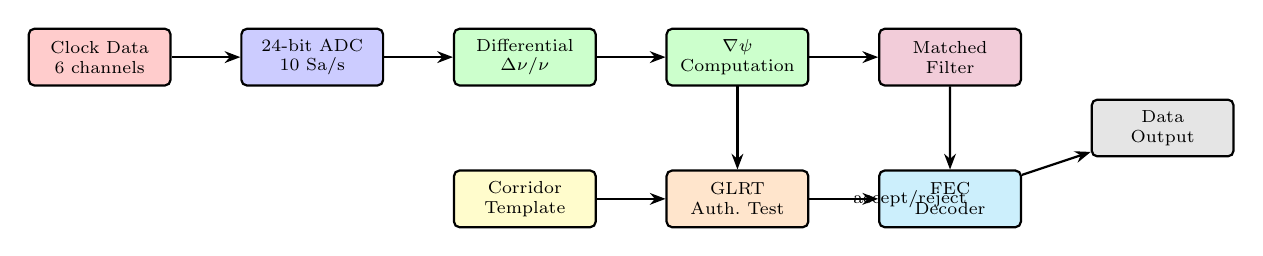
\begin{tikzpicture}[
  block/.style={draw, thick, minimum width=2cm, minimum height=0.8cm,
    rounded corners=2pt, align=center, font=\scriptsize},
  arr/.style={-{Stealth[length=2mm]}, thick},
  scale=0.9, transform shape
]

% Input
\node[block, fill=red!20] (clk) at (0,0) {Clock Data\\6 channels};

% ADC
\node[block, fill=blue!20] (adc) at (3,0) {24-bit ADC\\10~Sa/s};

% Diff
\node[block, fill=green!20] (diff) at (6,0) {Differential\\$\Delta\nu/\nu$};

% Gradient
\node[block, fill=green!20] (grad) at (9,0) {$\nabla\psi$\\Computation};

% GLRT
\node[block, fill=orange!20] (glrt) at (9,-2) {GLRT\\Auth.\ Test};

% Template
\node[block, fill=yellow!20] (tmpl) at (6,-2) {Corridor\\Template};

% Matched filter
\node[block, fill=purple!20] (mf) at (12,0) {Matched\\Filter};

% Decoder
\node[block, fill=cyan!20] (dec) at (12,-2) {FEC\\Decoder};

% Output
\node[block, fill=gray!20] (out) at (15,-1) {Data\\Output};

\draw[arr] (clk) -- (adc);
\draw[arr] (adc) -- (diff);
\draw[arr] (diff) -- (grad);
\draw[arr] (grad) -- (mf);
\draw[arr] (grad) -- (glrt);
\draw[arr] (tmpl) -- (glrt);
\draw[arr] (mf) -- (dec);
\draw[arr] (dec) -- (out);
\draw[arr] (glrt) -- node[right, font=\scriptsize] {accept/reject} (dec);

\end{tikzpicture}
\caption{Receiver signal processing pipeline.}
\label{fig:rx-pipeline}
\end{figure}

%=============================================================================
\section{Link Budget Analysis}
%=============================================================================

\subsection{Transmitter Output}

The $\psi$-field amplitude at the transmitter aperture, using the
parametric amplification channel:
\begin{equation}
\delta\psi_{\rm tx} = \frac{|\lambda - 1|\,\eta_\times\,U_0}
{M_\psi\,\Omega_\psi\,\gamma_\psi}.
\end{equation}

\begin{table}[H]
\centering
\caption{Link budget: transmitter side.}
\label{tab:tx-budget}
\begin{tabular}{lccc}
\toprule
Parameter & Symbol & Value & Unit \\
\midrule
EM--$\psi$ coupling & $|\lambda - 1|$ & $10^{-5}$ & --- \\
TE+TM overlap & $\eta_\times$ & 0.3 & --- \\
Stored energy & $U_0$ & $10^5$ & J \\
$\psi$-mode eff.\ mass & $M_\psi$ & $\sim 10^{-1}$ & kg$\cdot$m$^2$/s \\
$\psi$-mode frequency & $\Omega_\psi$ & $\sim 60$ & rad/s \\
$\psi$-mode damping & $\gamma_\psi$ & 0.03 & s$^{-1}$ \\
\midrule
Transmit $\psi$ amplitude & $\delta\psi_{\rm tx}$ & $\sim 10^{-2} |\lambda-1|$ & --- \\
 & & $\sim 10^{-7}$ & (for $|\lambda-1|=10^{-5}$) \\
\bottomrule
\end{tabular}
\end{table}

\textbf{Note:} The transmit amplitude depends critically on the true
value of $|\lambda - 1|$.
At the accidental bound ($3 \times 10^{-5}$), the transmit level is
$\delta\psi_{\rm tx} \sim 3 \times 10^{-7}$.
At a more conservative value ($10^{-10}$), the transmit level drops to
$\sim 10^{-12}$.

\subsection{Path Loss}

For a point-source-like $\psi$-generator, the field falls as $1/r$:
\begin{equation}
\delta\psi(r) = \delta\psi_{\rm tx}\,\frac{R_{\rm src}}{r},
\end{equation}
where $R_{\rm src}$ is the effective source radius.

The gradient falls as $1/r^2$:
\begin{equation}
|\nabla\psi(r)| = \delta\psi_{\rm tx}\,\frac{R_{\rm src}}{r^2}.
\end{equation}

\begin{table}[H]
\centering
\caption{Link budget: path loss.}
\label{tab:path-loss}
\begin{tabular}{lccc}
\toprule
Parameter & Value & Unit & Notes \\
\midrule
Source radius $R_{\rm src}$ & 0.3 & m & Cavity array extent \\
Link distance $L$ & 10 & m & Lab-scale demo \\
$\psi$ amplitude loss & $R_{\rm src}/L = 0.03$ & --- & 30~dB loss \\
$\psi$ gradient loss & $R_{\rm src}/L^2 = 0.003$ & m$^{-1}$ & 50~dB loss \\
\bottomrule
\end{tabular}
\end{table}

\subsection{Received Signal}

\begin{table}[H]
\centering
\caption{Link budget: received signal (for $|\lambda-1| = 10^{-5}$).}
\label{tab:rx-signal}
\begin{tabular}{lccc}
\toprule
Quantity & Value & Unit & Detector \\
\midrule
$\delta\psi_{\rm rx}$ & $\sim 10^{-8}$ & --- & Clock pair (differential) \\
$|\nabla\psi_{\rm rx}|$ & $\sim 10^{-9}$ & m$^{-1}$ & Clock gradiometer \\
$\Delta\nu/\nu$ (1~m baseline) & $\sim 5 \times 10^{-10}$ & --- & Easily detectable \\
\bottomrule
\end{tabular}
\end{table}

For $|\lambda - 1| = 10^{-10}$ (more conservative):
\begin{table}[H]
\centering
\caption{Link budget: received signal (for $|\lambda-1| = 10^{-10}$).}
\label{tab:rx-signal-conservative}
\begin{tabular}{lccc}
\toprule
Quantity & Value & Unit & Detection feasibility \\
\midrule
$\delta\psi_{\rm rx}$ & $\sim 10^{-13}$ & --- & Detectable in $\sim 10^4$~s \\
$|\nabla\psi_{\rm rx}|$ & $\sim 10^{-14}$ & m$^{-1}$ & Detectable in $\sim 10^4$~s \\
$\Delta\nu/\nu$ (1~m baseline) & $\sim 5 \times 10^{-15}$ & --- & Within clock capability \\
\bottomrule
\end{tabular}
\end{table}

\subsection{Noise Budget}

\begin{table}[H]
\centering
\caption{Noise budget at receiver.}
\label{tab:noise}
\begin{tabular}{lcc}
\toprule
Noise Source & Level & Mitigation \\
\midrule
Clock instability & $5 \times 10^{-17}/\sqrt{\tau}$ & Long integration \\
Fiber link noise & $< 10^{-19}$ & Active stabilization \\
Seismic/gravity gradient & $\sim 10^{-16}$~m$^{-1}$ at 0.1~Hz & Vibration isolation \\
Tidal variation & $\sim 10^{-17}$~m$^{-1}$ at diurnal & Subtracted in post-processing \\
EM interference & $< -80$~dB & Faraday cage \\
Thermal gradient & $\sim 10^{-19}$ & Temperature control \\
\bottomrule
\end{tabular}
\end{table}

\subsection{SNR Summary}

\begin{table}[H]
\centering
\caption{Signal-to-noise ratio summary ($\tau = 10^3$~s integration).}
\label{tab:snr}
\begin{tabular}{lccc}
\toprule
Scenario & $|\lambda-1|$ & SNR (amplitude) & SNR (gradient) \\
\midrule
Optimistic & $10^{-5}$ & $> 10^6$ & $> 10^4$ \\
Moderate & $10^{-8}$ & $\sim 10^3$ & $\sim 10$ \\
Conservative & $10^{-10}$ & $\sim 10$ & $\sim 0.1$ \\
Pessimistic & $10^{-12}$ & $\sim 0.1$ & $\sim 10^{-3}$ \\
\bottomrule
\end{tabular}
\end{table}

The demonstrator is viable for $|\lambda - 1| \gtrsim 10^{-10}$
with integration times of $\sim 10^3$--$10^4$~s per symbol.

%=============================================================================
\section{Test Plan}
%=============================================================================

\subsection{Test Sequence}

\begin{table}[H]
\centering
\caption{Test sequence.}
\label{tab:test-sequence}
\begin{tabular}{clcc}
\toprule
Test & Description & Duration & Success Criterion \\
\midrule
T1 & Noise floor characterization & 1 week & Noise matches model \\
T2 & $\psi$-generation (Tx ON, no data) & 2 weeks & $\delta\psi > 5\sigma$ \\
T3 & Template acquisition & 1 week & 5 points, SNR $> 3$ \\
T4 & Binary ASK transmission & 4 weeks & BER $< 10^{-3}$ \\
T5 & FSK transmission & 2 weeks & BER $< 10^{-3}$ \\
T6 & Gradient key switching & 2 weeks & Key discrimination $> 5\sigma$ \\
T7 & GLRT authentication & 2 weeks & $P_{\rm FA,spoof} < 10^{-3}$ \\
T8 & EM jamming resilience & 1 week & No BER degradation \\
T9 & Barrier penetration (optional) & 2 weeks & Data through barrier \\
\bottomrule
\end{tabular}
\end{table}

\subsection{Test T2: $\psi$-Generation Verification}

This is the critical first test.
Detailed protocol:

\begin{enumerate}
\item \textbf{Baseline:} Record receiver output for 24 hours with
transmitter OFF.
Compute power spectral density $S_0(f)$.

\item \textbf{Excitation:} Activate SRF cavity array with $2\omega$
modulation.
Record receiver output for 24 hours.
Compute power spectral density $S_1(f)$.

\item \textbf{Analysis:} Compute excess power at $\Omega_\psi$:
\begin{equation}
\Delta S = S_1(\Omega_\psi) - S_0(\Omega_\psi).
\end{equation}

\item \textbf{Decision rule:}
\begin{itemize}
\item $\Delta S > 5\sigma_S$: $\psi$-generation detected $\Rightarrow$
proceed to T3.
\item $\Delta S < 3\sigma_S$: Upper bound on $|\lambda - 1|$ $\Rightarrow$
increase integration, optimize coupling.
\end{itemize}

\item \textbf{Systematic checks:}
\begin{itemize}
\item Verify EM shielding (Faraday cage leakage test).
\item Verify no acoustic coupling (vibration monitor).
\item Rotate receiver orientation (distinguish $\psi$-gradient
from systematic).
\end{itemize}
\end{enumerate}

\subsection{Test T7: GLRT Authentication}

\begin{enumerate}
\item \textbf{Establish template:} Transmitter at position $\mathbf{r}_A$,
acquire fingerprint $\mathbf{F}_A$ over $N_s = 5$ points.

\item \textbf{Legitimate test:} Transmitter remains at $\mathbf{r}_A$,
transmit known sequence.
Compute $\Lambda$ for each symbol.
Verify $\Lambda < \eta$ for all symbols (acceptance).

\item \textbf{Spoofing test:} Move transmitter to
$\mathbf{r}_E = \mathbf{r}_A + \Delta\mathbf{r}$ with
$|\Delta\mathbf{r}| = 1$~m, 2~m, 5~m.
Transmit identical sequence.
Compute $\Lambda$ for each symbol.
Verify $\Lambda > \eta$ for spoofed symbols (rejection).

\item \textbf{Metrics:}
\begin{itemize}
\item False rejection rate (legitimate rejected): target $< 10^{-3}$.
\item False acceptance rate (spoofed accepted): target $< 10^{-3}$.
\item ROC curve: $P_{\rm FA}$ vs.\ $P_{\rm D}$ as function of
$|\Delta\mathbf{r}|$ and $N_s$.
\end{itemize}
\end{enumerate}

%=============================================================================
\section{Risk Assessment}
%=============================================================================

\begin{table}[H]
\centering
\caption{Risk register.}
\label{tab:risks}
\begin{tabular}{p{0.25\textwidth}ccp{0.35\textwidth}}
\toprule
Risk & Likelihood & Impact & Mitigation \\
\midrule
$|\lambda - 1| = 0$ (no EM--$\psi$ coupling) & Medium & Critical &
Fall back to gravitational $\psi$-generation (moving masses); redesign
transmitter. \\
\addlinespace
$|\lambda - 1| < 10^{-12}$ (coupling too weak) & Medium & High &
Increase integration time; upgrade to MAGIS-class atom interferometer
detector. \\
\addlinespace
Seismic noise dominates & Low & Medium &
Deploy in quiet underground facility; use Newtonian noise subtraction. \\
\addlinespace
EM leakage through shield & Low & High &
Pre-test shielding effectiveness; add active cancellation. \\
\addlinespace
$\psi$-mode frequency unknown & Medium & Medium &
Scan $2\omega_{\rm mod}$ across expected range; use broadband detection. \\
\addlinespace
Clock systematics mask signal & Low & Medium &
Use multiple clock species (Sr, Yb) for cross-check. \\
\bottomrule
\end{tabular}
\end{table}

%=============================================================================
\section{Cost and Schedule Estimate}
%=============================================================================

\subsection{Cost Breakdown}

\begin{table}[H]
\centering
\caption{Estimated cost breakdown (order-of-magnitude).}
\label{tab:cost}
\begin{tabular}{lcc}
\toprule
Item & Cost (USD) & Notes \\
\midrule
SRF cavity array (4 cavities) & \$4M & Repurpose existing cavities \\
Cryogenic system (2~K) & \$2M & Standard He plant \\
RF drive and LLRF system & \$500K & Existing designs \\
Optical clock pair (6 units) & \$6M & State-of-the-art \\
SQUID gradiometer array & \$500K & Commercial \\
Faraday cage and shielding & \$200K & Custom fabrication \\
Vibration isolation & \$100K & Commercial \\
Signal processing electronics & \$200K & FPGA + ADC/DAC \\
Integration and commissioning & \$500K & Engineering labor \\
\midrule
\textbf{Total} & \textbf{\$14M} & \\
\bottomrule
\end{tabular}
\end{table}

\subsection{Schedule}

\begin{table}[H]
\centering
\caption{Project schedule.}
\label{tab:schedule}
\begin{tabular}{clc}
\toprule
Phase & Activity & Duration \\
\midrule
1 & Design finalization and procurement & 6 months \\
2 & SRF cavity preparation and test & 12 months \\
3 & Receiver assembly and calibration & 12 months \\
4 & System integration & 6 months \\
5 & Testing campaign (T1--T9) & 12 months \\
\midrule
& \textbf{Total} & \textbf{4 years} \\
\bottomrule
\end{tabular}
\end{table}

%=============================================================================
\section{Alternative and Reduced-Cost Configurations}
%=============================================================================

\subsection{Configuration B: Single Cavity + Single Clock Pair}

A minimal demonstration using:
\begin{itemize}
\item 1 SRF cavity (100 kJ stored energy),
\item 1 optical clock pair (1~m baseline),
\item Reduced shielding.
\end{itemize}

Estimated cost: \$3M.
Capability: Tests T1, T2, T4 only (no gradient mapping or authentication).

\subsection{Configuration C: Gravitational $\psi$-Source}

If $|\lambda - 1| = 0$ (no EM--$\psi$ coupling), the fallback is
a mechanical $\psi$-generator using moving masses:
\begin{itemize}
\item Rotating tungsten mass ($M = 500$~kg, $R = 0.5$~m, $f = 10$~Hz).
\item $\psi$-perturbation:
$\delta\psi = 2GM/(c^2 R) \approx 7 \times 10^{-25}$.
\item Gradient at 1~m:
$|\nabla\psi| \approx 2GM/(c^2 R^2) \approx 7 \times 10^{-25}$~m$^{-1}$.
\end{itemize}
This is below current detection thresholds and would require
next-generation gravitational sensors.

\subsection{Configuration D: Hybrid EM/$\psi$ Demonstration}

Instead of pure $\psi$-communication, demonstrate the hybrid concept:
\begin{itemize}
\item $\psi$-corridor provides timing reference.
\item EM signal (optical fiber or free-space laser) provides data payload.
\item Receiver verifies EM arrival time against $\psi$-corridor delay.
\end{itemize}
This requires only $\psi$-detection (not $\psi$-modulation) and is
achievable with existing gravitational sensor technology.

%=============================================================================
\section{Conclusion}
%=============================================================================

This engineering design specifies a laboratory-scale $\psi$-field
communication demonstrator capable of validating the core claims of
Patent \#8.
The critical path item is the unknown value of $|\lambda - 1|$: the
EM--$\psi$ coupling parameter determines whether the demonstrator
operates in the high-SNR regime ($|\lambda - 1| \sim 10^{-5}$, trivially
detectable) or the low-SNR regime ($|\lambda - 1| \lesssim 10^{-12}$,
requiring extended integration).

The system is designed to be viable across this entire range:
\begin{itemize}
\item For $|\lambda - 1| \gtrsim 10^{-8}$: Full demonstration of ASK
data transfer, gradient mapping, and GLRT authentication is achievable
within $10^3$~s integration per symbol.
\item For $10^{-12} \lesssim |\lambda - 1| \lesssim 10^{-8}$: $\psi$-generation
is detectable; communication requires $10^4$--$10^6$~s per symbol.
\item For $|\lambda - 1| \lesssim 10^{-12}$: Only $\psi$-generation
upper bounds are achievable; fall back to Configuration C or D.
\end{itemize}

The estimated cost of \$14M for the full configuration is comparable
to a mid-scale physics experiment and leverages existing SRF and atomic
clock infrastructure.
The reduced Configuration B at \$3M provides a cost-effective first
step toward $\psi$-generation verification.

\end{document}
